% =====================================================================
%  Chapter 20 — \idxw{Interferometry}, \idxw{Visibility} and the Over-Resolution\idx{Over-resolution} Limit
% =====================================================================

\chapter{Interferometry, Visibility and the Over-Resolution Limit}
\label{ch:interferometry}

Interferometry\idx{Interferometry} is the only method in the field that can resolve a small
object without going near it, because the resolution it delivers is set by
the baseline rather than by the distance. It is also the method whose
design literature is, on the evidence of the book's own re-derivation,
sized for the wrong objects. This chapter works out what an asteroid shape
imager actually requires.

\section{The fringe spacing and the sampling condition}

Two apertures separated by a baseline \(B\), observing at wavelength
\(\lambda\), receive the same wavefront with a path difference that varies
across the field. The angle at which the path difference is one wavelength
is the fringe spacing
\begin{equation}
\theta_{\mathrm{fs}} = \frac{\lambda}{B}.
\label{eq:fringe}
\end{equation}
For a body of angular diameter \(\theta_{\mathrm{diam}}\), the number of
fringe spacings across the body is
\begin{equation}
N = \frac{\theta_{\mathrm{diam}}}{\theta_{\mathrm{fs}}}
= \frac{\theta_{\mathrm{diam}}\, B}{\lambda},
\label{eq:samples}
\end{equation}
and the body is imaged when \(N\) is of order four or more.

Four is not arbitrary. The 3 Juno image made with the Atacama Large
Millimeter Array resolved a body 180 milliarcseconds across at an angular
resolution of 0.042 arcseconds, which is 4.3 samples across the diameter.
The book's generator uses that as the calibration for the condition, and
Appendix A gives the full re-derivation.

\begin{table}[!htbp]
\centering
\small
\caption{The baseline required for four samples across the diameter, at
750 nanometres, for the class of interest.}
\label{tab:required-baseline}
\begin{tabularx}{\textwidth}{@{}P{0.60in}P{0.66in}P{0.67in}P{0.66in}Y@{}}
\toprule
\rowcolor{panel}
\textbf{Diameter} & \textbf{Distance} & \textbf{Angular size} &
\textbf{Baseline} & \textbf{At 0.1 AU} \\
\midrule
60 m & 0.1 AU & 0.83 mas & 748 m & 1,496 m \\
\rowcolor{panel}
60 m & 0.2 AU & 0.41 mas & 1,496 m & 3,740 m \\
60 m & 0.5 AU & 0.17 mas & 3,740 m & 13,090 m \\
\rowcolor{panel}
140 m & 0.1 AU & 1.93 mas & 321 m & 561 m \\
140 m & 0.2 AU & 0.97 mas & 641 m & 1,122 m \\
\rowcolor{panel}
140 m & 0.5 AU & 0.39 mas & 1,603 m & 2,805 m \\
\bottomrule
\end{tabularx}
\end{table}

\tabref{tab:required-baseline} is the book's most consequential table. The
required baselines are hundreds of metres to kilometres. They are not
hundreds of kilometres, and they are not tens of metres.

\begin{figure}[!htbp]
\centering
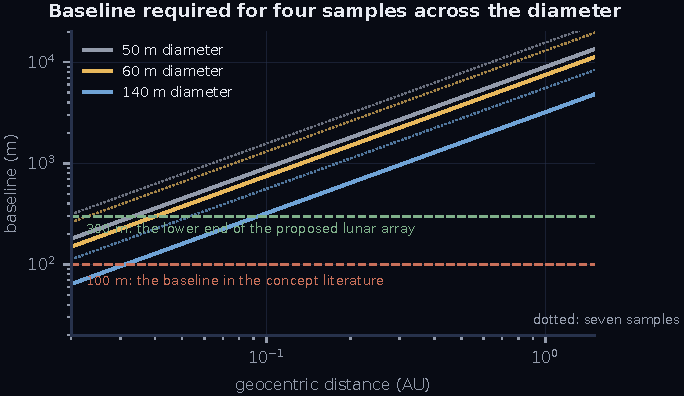
\includegraphics[width=\textwidth]{../figures/fig_shape_baseline.pdf}
\caption{The baseline required for four samples across the diameter, against
the geocentric distance, for three diameters. The 100-metre baseline of the
concept literature never reaches the requirement for the small class.}
\label{fig:shape-baseline}
\end{figure}

\section{The re-derivation of the concept study's own table}

The 2003 concept study for the Comet/Asteroid Protection System published a
table of the maximum baseline usable against a target's angular size, for
eight cases spanning a one-kilometre object at six astronomical units and a
50-metre object at 0.2 astronomical units.

The book's generator reproduces that table's maximum-baseline column from
the rule
\begin{equation}
B_{\max} = \frac{\lambda}{4\,\theta_{\mathrm{diam}}},
\label{eq:bmax}
\end{equation}
to within 0.71 per cent on all eight rows, and reproduces the precision
column as
\begin{equation}
\sigma_\theta = \frac{\lambda}{B\,\mathrm{SNR}}
\label{eq:precision}
\end{equation}
to within 2.21 per cent, with the signal-to-noise ratio of 7 given in the
source.

That the table reproduces does not mean the table is right for the purpose
the book needs. It means the table is internally consistent, and its
consistency lets us read off what it is actually describing.

\section{What the design point actually is}

The concept study's design point is a 100-metre baseline with three-metre
apertures at 750 nanometres, a fringe visibility of 0.5 and a visual
magnitude of 27.

Apply \eqref{eq:samples} to a 50-metre object with that baseline. At 0.1
astronomical units the object's angular diameter is 0.689 milliarcseconds
and the fringe spacing is 1.547 milliarcseconds, so
\begin{equation}
N = \frac{0.689}{1.547} = 0.45.
\end{equation}
At 0.2 astronomical units the angular diameter is 0.345 milliarcseconds and
the ratio is 0.22. In both cases \textbf{the target is smaller than half of
one fringe spacing}. The instrument is an astrometric centroid, and the
concept study says so itself: its stated purpose is ``a commensurate drop in
the orbit determination error''.

\begin{seamnote}{The 2024 and 2025 lunar interferometry literature is sized
for stars}
The recent lunar optical interferometry study proposes a 100-metre baseline
with 30-centimetre apertures over 450 to 850 nanometres, and the
Artemis-enabled stellar imager is a long-baseline ultraviolet and optical
instrument for stellar astrometry. Both are sized for milliarcsecond stellar
astrometry, and neither is an asteroid shape imager. Neither was intended to
be. The point of the re-derivation is not to accuse them of an error; it is
to establish that the lunar shape-imaging niche is unoccupied by the
literature, and that its baseline requirement is a kilometre-scale one.
\end{seamnote}

\begin{figure}[!htbp]
\centering
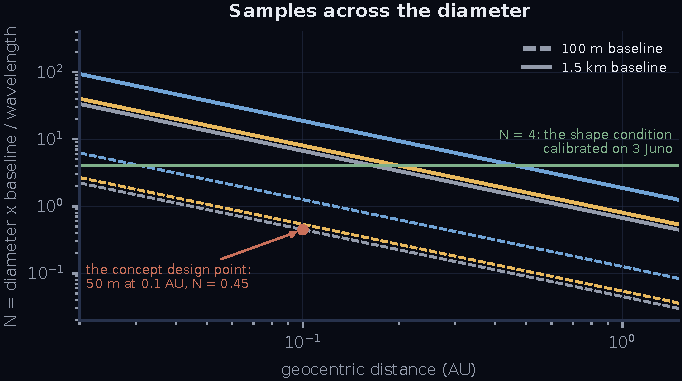
\includegraphics[width=\textwidth]{../figures/fig_samples.pdf}
\caption{Samples across the diameter against baseline and distance. A
hundred-metre baseline never reaches four samples for the 50-metre class at
0.2 astronomical units; a 1.5-kilometre baseline reaches it comfortably
across most of the class's distance range.}
\label{fig:samples2}
\end{figure}

\section{Visibility, and the over-resolution limit}

The other limit is the opposite one. A baseline much longer than the body
requires produces fringes whose visibility collapses, because the body's own
structure, rather than the instrument, then sets the visibility. The
uniform-disc model gives the visibility as
\begin{equation}
V = \left|\frac{2 J_{1}(x)}{x}\right|,
\qquad
x = \frac{\pi B\,\theta_{\mathrm{radius}}}{\lambda},
\label{eq:visibility}
\end{equation}
which the generator evaluates with the convergent series for the Bessel
function.

This is the over-resolution limit, and it is the reason the required baseline
must be \emph{matched} to the target rather than simply made long. The
usable baseline window for a target of a given angular size is bounded on
both sides: too short and the body is unresolved, too long and the fringe
visibility is gone.

\begin{table}[!htbp]
\centering
\small
\caption{The usable baseline window for the small class at 750 nanometres,
with four samples as the lower bound and a unit visibility as the upper.}
\label{tab:baseline-window}
\begin{tabularx}{\textwidth}{@{}P{0.77in}P{0.89in}P{1.04in}Y@{}}
\toprule
\rowcolor{panel}
\textbf{Diameter} & \textbf{Distance} & \textbf{Baseline window} &
\textbf{Comment} \\
\midrule
60 m & 0.2 AU & 1.5 to 1.9 km & the narrowest useful window in the class \\
\rowcolor{panel}
60 m & 0.5 AU & 3.7 to 4.4 km & \\
140 m & 0.2 AU & 0.6 to 0.8 km & \\
\rowcolor{panel}
140 m & 0.5 AU & 1.6 to 1.9 km & \\
\bottomrule
\end{tabularx}
\end{table}

The windows in \tabref{tab:baseline-window} are the reason the architecture
has to be an array with a choice of separations rather than a single
interferometer. A station that has to image a 60-metre object at 0.2
astronomical units and a 140-metre object at 0.5 astronomical units needs
baselines of very different lengths, and it needs to be able to select
between them on the timescale of a campaign.

\begin{deeper}{The visibility model this book does not have}
\eqref{eq:visibility} is a uniform-disc model, and the book says plainly
that it is not adequate for the resolved case. A genuinely resolved body
with limb darkening and surface contrast produces a visibility that is not
the uniform-disc function at all, and the fringe visibility of a real
asteroid at a matched baseline is a property of its albedo distribution
across the disc. The requirement for four samples is insensitive to this,
because it is set by the sampling condition rather than by the visibility.
The \emph{achievable precision} is not insensitive, and the book does not
claim a calibrated precision for a resolved target. What it does claim is
the requirement, which is what a programme would be specified against.
\end{deeper}

\begin{keytakeaways}
\item A shape image requires four samples across the diameter, which for the
60-metre class means baselines of 748 metres at 0.1 astronomical units and
3,740 metres at 0.5.
\item The concept study's own table reproduces as \(B_{\max} = \lambda/(4
\theta)\) to within 0.71 per cent, and its 100-metre design point puts the
50-metre class below half a fringe spacing.
\item The recent lunar interferometry literature is sized for stellar
astrometry, which leaves the asteroid shape-imaging niche unoccupied.
\item The usable baseline window is bounded on both sides, so the station has
to be an array with selectable separations rather than a single
interferometer.
\end{keytakeaways}
